\pagelayout{margin}
\setchapterstyle{kao}
\setchapterpreamble[u]{\margintoc}

\chapter{Related research}

This chapter reviews literature on electric vehicle (EV) charging demand prediction and related methodologies, providing context for our research on charging patterns in Prague.

We examine four main research areas: data-driven approaches to understanding charging behavior, simulation-based methodologies for predicting demand, stochastic modeling approaches capturing probabilistic behavior, and research specific to the Czech context. The review highlights spatial and temporal dimensions of charging demand, data requirements of different approaches, and trade-offs between model complexity and accuracy.

This analysis identifies gaps in existing research regarding Prague's urban environment and informs our methodological approach.



\subsection{Understanding EV Charger Use by Data}

To understand why certain chargers are being utilized the way they are. Research utilizes traditional and Bayesian statistics. As the person that plans \acrfull{CP} it is good to have insight into what influences charging demand. That is, why a certain charger is utilized. And what factors contribute to it. So far, we dont care about expansion of the infrastrcture. But could provide insights that allow to place new chargers more strategically.

\sidecite{hechtGlobalElectricVehicle2024} gathered counts of types of \acrfull{POI}\sidenote{types like shops, sport areas, schools, offices} near every charger of interest \sidenote{Search radius of 2000m around each charger with linear decrease in importance in relation to distance} from Open Street maps. Then for each charger computed its utilization. Which is its average daily power consumption. Then used linear regression to test which of the category of \acrfull{POI} contributed to the consumption.
The study had some statisficaly significant results. They also trained neural network model for capturing non linear relationships. User can use the model to select any point where a \acrfull{CP} might be placed and see its estimated utilization and evaluate worthiness of placement. However it does not work with other chargers in the area and does take into account charger density. The paper has identified that certain categories of \acrfull{POI}\sidenote{\acrshort{POI} data obtained from OpenStreetMaps} are correlated with charger demand.

\sidecite{dongElectricVehicleCharging2019} uses log-Gaussian Cox process. Which is a statistical model that can handle dependence between points on a map (EV chargers). It has identified that workplace population and traffic flow are positively related to demand of\acrfull{CP} while commerce is in a negative relation. \sidenote{<workplace population, traffic flow, commerce description here>}.

\begin{kaobox}[frametitle=Simulation vs Model]
    Model is concerned with representing a system of interest. Purpose of it is so it matches its real system in some behaviour while being simpler than reality. There are many ways how to construct models. From simplest small replicas (small car models to use in wind tunnel) to complicated mathematical and software ones.

    Simulation is then a use of model to try to replicate some real system of interest to gain insights how a real system might behave .

    An example can be a toy car and a ramp which would be our model. Then pushing the car off the ramp to see how far it is able to land. This is much less expensive than pushing real cars of larger ramps.

    \cite{maria1997introduction}
\end{kaobox}

\subsection{Simulations and EV Charger Use}

\textbf{Trafic models} are used to estimate \acrfull{CP} demand. They are a mathematical model of real-world trafic. And they can estimate charging demand by introducting EV vehicle agents into the simultion. Those agents navigate replica of real road network. While also being able to emulate traffic jams, alternative path finding. Negative of these models is that they are harder to develop, fine tune to match real situation. And performance costly. But once developed and validated with real-world. They can be highly utilized.

\begin{kaobox}[frametitle=\text{Micro,Macro,Meno-Scopic}]

    Traffic models can be separated into three groups according to \cite{TrafficAnalysisTools}\cite{HomeAustroads}(\cite{lachowiczMicroscopicMesoscopicMacroscopic2011} also writes about splitting simmulation models into 3 groups with a more theoretical view):

    % \todo{improve, im actually not really sure about the difference of mesoscopic vs rest}
    \begin{itemize}
        \item \textbf{Microscopic} - Simulation of individual agents/vehicles. Can be as detailed as emulating accelerating, lane changing, turning. Higher fidelity isuUsable for example when designing intersection with light signals optimizing for traffic or pedestrian flow. But the model can also have less detailed fidelity for vehicles. Which simplifies the simmulation and enables larger area of interest. Like cities or even countries.
        \item \textbf{Mesoscopic} - Provide less fidelity than microscopic. improve
        \item \textbf{Macroscopic} - Work with aggregate information. Work more on analytical model and proven mathematcial relationships between traffic flow. improve
    \end{itemize}
\end{kaobox}


Matsim \sidecite{communityMATSim2025} is \acrfull{ABM} \marginnote{Slight foreshadowing but this approach was not taken in this thesis however it was considered.}. It's OpenSource software licensed under GPLv2, implemented in Java. And started in 2004 in Zurich. It falls into category of microscopic models due to it being able to simluate individual agents. The model simmulates simplifed version of vehicle movement and traffic which is needed to correctyl simulate entire city including congestions. The simulation usually concerns only one day. To create such a model the following are needed:
\begin{itemize}
    \item \textbf{Road/communication Network} - Spatial data for area of interest reagarding: roads, intersections, tram or train tracks etc. Obtained from technical data published by goverments or third party map providers. (Mainly OpenStreetMaps)
    \item \textbf{Population} - Agents with their day plan, where are they going to live and commute to work. Those are generated with help of expert knowledge and travel diaries survey.
    \item \textbf{Facilities} - Locations where activities can be performed. Obtained from third parties like OpenStreetMaps.
\end{itemize}

\begin{figure}
    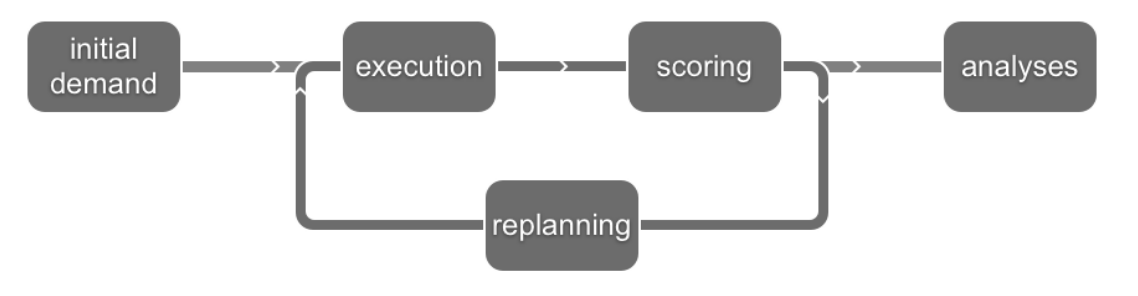
\includegraphics{matsim-simmulation-stages.png}
    \caption[Matsim, Simulation stages]{Stages of matsim simulation. \cite{Horni2016}}
    \labfig{matsim-simulation}
\end{figure}

The agents plan assigns unique daily schedule for each agent in the population. See \ref{fig:matsim-simulation} This estabilished the initial demand. During the execution step, Matsim simulates agents commute and tries to satisft the agents schedule. The agent might fail to be on schedule due to road or public transport congestion from other agents. After finishing the simulation the agents actual daily schedule is scored. Penalizing arriving at work late or being stuck for too long in traffic giving agents lover score. While agents who got where they wanted qucikly and without trafic jams get better score. During replanning agent schedule can be modified so it either adjusts the agents schedule, like less time spent home or taking a different route to work. When the simulation is sufficiently optimized the results of it can be then used for various analysis as the output of the modle is detailed log of agent activities.

\begin{marginfigure}
    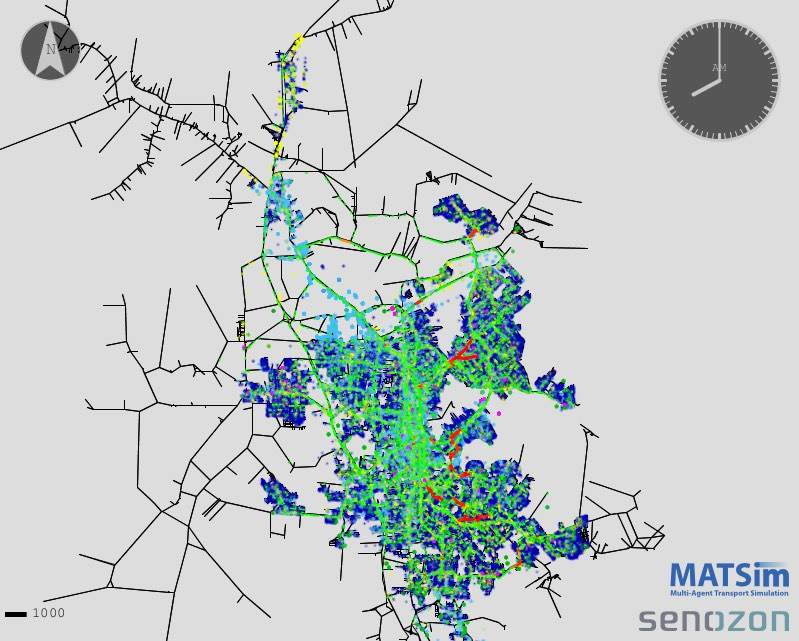
\includegraphics{joinville_1.jpg}
    \caption[Matsim, Joinville example]{Matsim, Joinville example. Model intended to help the city encumbered by high traffic volumes.\\
        \url{https://matsim.org/gallery/joinville/}}
    \labfig{joinville_example}
\end{marginfigure}

To create the agents schedule, day intentions need to be provided to the model. Those can be either manually crafted. With the increased availabiliy of census data, data driven approach can be taken. This trades away the possibility to experiment with different kinds of populations and policies\sidenote{like exmaining effect of different school time start on traffic} but simplifies the process of creation where only data is needed and not expert knowledge on human behavior. \sidecite{drchalDatadrivenActivityScheduler2019} models multiple probability densities for what activity will an agent do, how long it will take and what activities are available in the area. This utilizies several datasets. New schedules can be generated from the model by sampling from the distributions.

Finaly, moving to use of Matsim for ev scenarios. \sidecite{novoselAgentBasedModelling2015} studies the impact of EVs on the electric id and electricty production in Croatia. By having a simmulation of power production network for the whole country as well. They first have a simmulation regarding the current state and how that impacts the electrical grid. This sets the baseline and also allows to correctly calibrate the model. Then they increase the ev adoption and see what is the hourly energy consumption of EVs and their impact on the grid.

\textbf{Stochastic models} provide a way for modeling charging behavior of electric vehicles by capturing randomness and uncertainty in travel patterns. They work with more simplified representation fo reality compared traffic models\sidenote{Of course trafic models have large part of stochasticity inside themselves}. These models typically employ probability distributions to characterize variables such as departure times, travel distances, parking durations, and charging decisions. By sampling from these distributions using techniques like Monte Carlo simulation, they generate synthetic power demand profiles.

\sidecite{bradyModellingChargingProfiles2016} presents an example of stochastic modeling applied to EV charging behavior. Their approach uses a non-parametric copula function to model the dependence structure between six variables: departure time, number of journeys, and total distance traveled across two consecutive days. For this they utilize real-world GPS data collected from electric vehicles. Their model simulates complete journey schedules for individual vehicles and implements a probabilistic charging decision model at each destination, conditioned on the state of charge, parking time, and journey number. The approach captures the variability in charging behavior by incorporating factors such as battery characteristics and probabilistic charging point availability.

\sidecite{ul-haqProbabilisticModelingElectric2018} presents a probabilistic model for EV charging patterns in residential networks. The authors employ a stochastic approach using Markov chains to model transitions between driving, parked, and charging states. Their model accounts for various factors such as vehicle type, battery capacity, state of charge, driving habits, and charging preferences. By simulating daily activity patterns across different seasons and day types, they estimate charging needs for various EV penetration levels (34\%, 50\%, 65\%). Results show distinct charging patterns between weekdays and weekends, with weekend peaks occurring later in evenings. This estimation of charging load patterns provides valuable insights for distribution network planning and management.



\begin{marginfigure}
    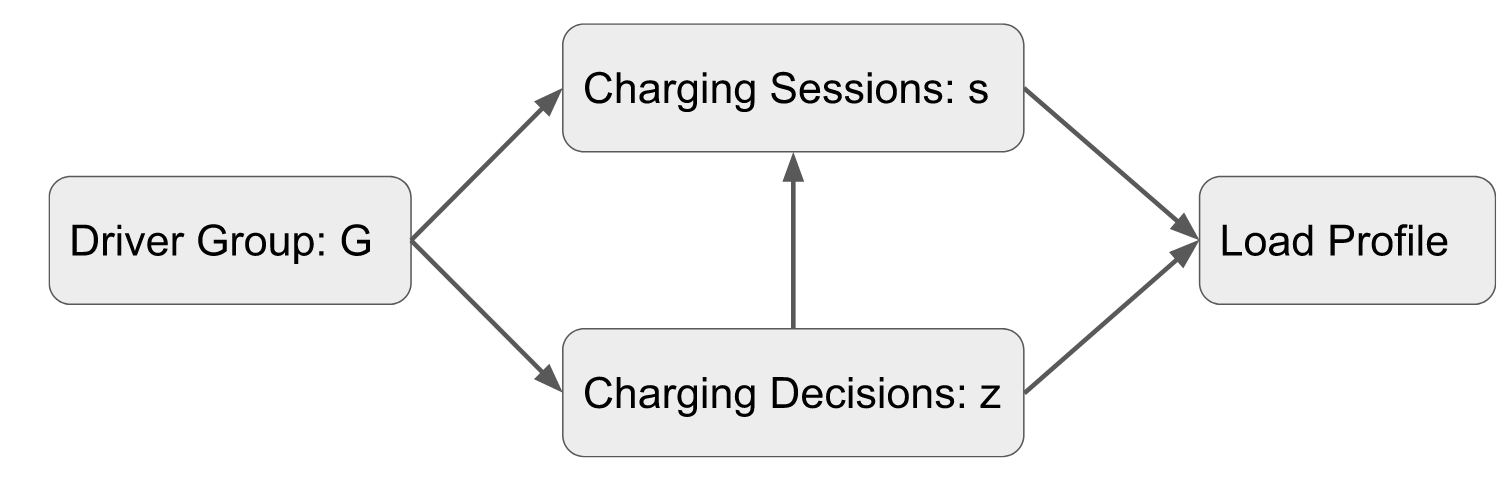
\includegraphics{powell_graphical_model.png}
    \caption{Graphical model of modelling EV driver charging behaviour \cite{powellChargingInfrastructureAccess2022}}
    \label{fig:powell_graphic_model}
\end{marginfigure}

\sidecite{powellScalableProbabilisticEstimates2022} utilizes graphical model. It breaks down the problem into modelling several probability distributions. They posessed charging sessions data with anonymized car ids. With the car ids they reconstructed drivers charging behaviour. They constructed vector encoding the drivers charging history and then aplied hierachcical clustering to group drivers into groups based on their behavior. They separated the chargers into 6 segments based on the charging power and its location (single family house, multi unit dwelling, workplace, fast charger). Then modelled the groups probability distribution of charging at the segments (see the graphical model at Figure \ref{fig:powell_graphic_model}). Then by sampling from the distribution they were able to reconstruct the power demand profile. And importanlty, see the effect by changing the amount of drivers in the identified driver groups. Being beneificial to policy makers.


% \begin{itemize}
%     \item \sidecite{zhangChargingDemandPrediction2023}
%     \item \sidecite{zhangUrbanChargingLoad2024}
% \end{itemize}


% \section{Forecasting}
% \todo{mention difference forecasting vs modelling}

% \textit{ML for predictions, not explainable. Just learning on data}

% \todo[inline]{This section contains only placeholder text and a todo note. It needs to be fully developed with a comprehensive review of forecasting approaches in EV charging demand literature, including both statistical forecasting methods and machine learning approaches. Include a discussion of the trade-offs between model explainability and predictive performance.}

% \section{Infrastructure Planning}

% \textit{Charger placement, optimization problem how to cover certain areas. ILP and others used}

% \todo[inline]{This section also contains only placeholder text. Develop a comprehensive review of infrastructure planning approaches, including optimization methods, coverage models, and decision support systems. Discuss how these approaches relate to your research on charging demand prediction.}


\section{Relevant Research for Czechia}

\sidecite{pekarekModelChargingService2017} introduces a standalone model for electric vehicle charging demand based on large-scale travel survey data from the Czech Republic. The model serves as a comprehensive input for subsequent charging infrastructure optimization problems. It develops a graph-based representation of the road network where traffic data is transformed from edge-defined to vertex-defined format. This mathematical approach allows for the introduction of a point-defined (vertex-defined) charging demand model where each road intersection (vertex) has an associated demand value.

The model utilizes real traffic survey data to determine the spatial distribution of charging demand, calculating how demand at specific points is influenced by traffic patterns in surrounding areas. This is accomplished through a distance diminishing function that propagates demand through the network while simulating driver behavior. It applies this model to the entire Czech Republic road network (comprising over 30,000 road segments) and identifies several limitations, particularly related to data availability in municipal areas and potential calculation inaccuracies in regions with high-density road networks.

\sidecite{neumannOptimalniRozmisteniNabijecich2021} focuses on optimization of charger placement in Czechia but on a private land.

\sidecite{elomiyaAdvancedSpatialDecision2024} focuses on detemrining the best placement of hydrgoen refill station. By using GIS multi-criteria decision making.  By taking into account criteria such as: proximity to junctions, flood prone areas, flat terrain, safety distance from selected area types and high population area. They did not posess data about the existing hydrogen

% \section{Data sources and transformations}
% estimate population

% Predicts density of each building per $100m^2$ living area. With $R^2 = 94\%$.
% \sidecite{shangEstimatingBuildingscalePopulation2021}

\section{Discussion}

The literature review reveals several distinct approaches to modeling and predicting EV charging demand, each with its own strengths and limitations.

Simulation-based approaches, particularly traffic models and agent-based models like MATSim, offer high flexibility and the ability to model complex interactions between vehicles, infrastructure, and human behavior. These models are valuable in data-scarce environments where empirical charging data is limited or non-existent. The work by \cite{novoselAgentBasedModelling2015} demonstrates how such simulations can be extended beyond charging demand prediction to assess impacts on electrical grids. However, these approaches require significant computational resources, expert knowledge for calibration, and extensive input data about road networks, population characteristics, and travel patterns.

In contrast, stochastic models like those presented by \cite{bradyModellingChargingProfiles2016} and \cite{ul-haqProbabilisticModelingElectric2018} offer a more data-driven approach while still capturing the inherent variability in charging behavior. These models typically employ probability distributions to characterize key variables such as departure times, travel distances, and charging decisions. The graphical model approach by \cite{powellScalableProbabilisticEstimates2022} is particularly noteworthy for its ability to identify distinct driver groups and model their charging behaviors separately, enabling more nuanced policy analysis.

The Czech-specific research by \cite{pekarekModelChargingService2017} provides valuable insights into modeling charging demand in the Czech Republic using a graph-based representation of the road network. However, this approach focuses on the national level and does not address the unique urban characteristics of Prague.

Several patterns emerge from this literature review:

\begin{enumerate}
    \item As data availability increases, research tends to shift from simulation-based approaches toward more data-driven statistical and machine learning methods. This progression reflects the natural evolution of research in emerging domains, where initial exploratory models based on expert knowledge gradually give way to empirical models as more data becomes available.

    \item Stochastic models that capture the probabilistic nature of human decision-making processes have proven effective in modeling charging behavior. These models can represent the inherent uncertainty in factors such as arrival times, charging durations, and energy consumption patterns.

    \item The spatial context of charging stations significantly influences their usage patterns, with factors such as proximity to workplaces, commercial areas, and transportation hubs playing important roles in determining charging demand.

    \item Temporal patterns in charging behavior exhibit distinct variations across different days of the week and seasons, necessitating models that can capture these cyclical patterns.
\end{enumerate}

The methodological approaches in the literature also reveal a clear trade-off between model complexity and data requirements. Simulation-based approaches like MATSim require extensive configuration and calibration but can operate with limited charging data, making them suitable for early-stage planning when empirical data is scarce. Conversely, data-driven approaches like those employed by \cite{powellScalableProbabilisticEstimates2022} and \cite{hechtGlobalElectricVehicle2024} require substantial historical charging data but can potentially deliver more accurate predictions with less configuration effort.